
\documentclass{article} % For LaTeX2e
\usepackage{iclr2027_conference,times}

% Optional math commands from https://github.com/goodfeli/dlbook_notation.
\input{math_commands.tex}

\usepackage{hyperref}
\usepackage{url}
\usepackage{amsmath,amssymb}
\usepackage{booktabs}
\usepackage{graphicx}
\usepackage{array}
\usepackage{algorithm}
\usepackage{algpseudocode}
\usepackage{tikz}
\usetikzlibrary{arrows.meta,positioning,fit,calc}
\graphicspath{{figs/}{./}}

\DeclareMathOperator*{\argmaxop}{arg\,max}
\DeclareMathOperator{\Dec}{Dec}
\DeclareMathOperator{\sgop}{sg}
\newcommand{\fitbox}[1]{\resizebox{\ifdim\width>\linewidth\linewidth\else\width\fi}{!}{#1}}
\newcommand{\naive}{naive CD}

\title{Scored Consistency Distillation of SD3.5-Medium\\with a Decode-Free Photographic Reward}

\author{Anonymous Author(s) \\ Affiliation \\ Address \\ \texttt{email}}

%\iclrfinalcopy % Uncomment for camera-ready version, but NOT for submission.
\begin{document}

\maketitle

% Every number in this document is produced from the raw evaluation records by iclr2027/verify_numbers.py
% (-> numbers.json) and typeset by iclr2027/make_tables.py (-> tables/*.tex) and make_paper_figures.py (-> figs/).

\section{Method}
\label{sec:method}

We distil SD3.5-Medium, a 2.5B-parameter rectified-flow transformer, into a 4-step student with no
classifier-free guidance. Consistency distillation (CD) trains the student to reproduce the teacher's
sampling trajectory. The naive recipe rolls out one teacher trajectory per caption and regresses onto it.
Our recipe changes two things and nothing else (Figure~\ref{fig:overview}):
\begin{enumerate}
\item \textbf{Scored trajectory selection.} For every training caption the frozen teacher produces four
  candidate trajectories, each is decoded and compared with the real photograph the caption was written
  for, and the student is trained only on the candidate that is closest to the photograph.
\item \textbf{A decode-free photographic reward.} During training a small projector network $P_\phi$
  maps the student's own clean-latent prediction straight into the image-embedding space used for
  scoring, so a photographic similarity reward is available on every update without decoding. Because the
  student's predictions drift away from the teacher's candidates that $P_\phi$ was pretrained on, $P_\phi$
  is briefly refit every 100 updates on decoded recent predictions.
\end{enumerate}
Both parts use the same quantity, the DINOv2 similarity between an image and the caption's photograph;
neither reads the caption text, a VLM or a learned preference model. At inference nothing remains but a
single 4-step network.

\begin{figure}[!htb]
\centering
\fitbox{%
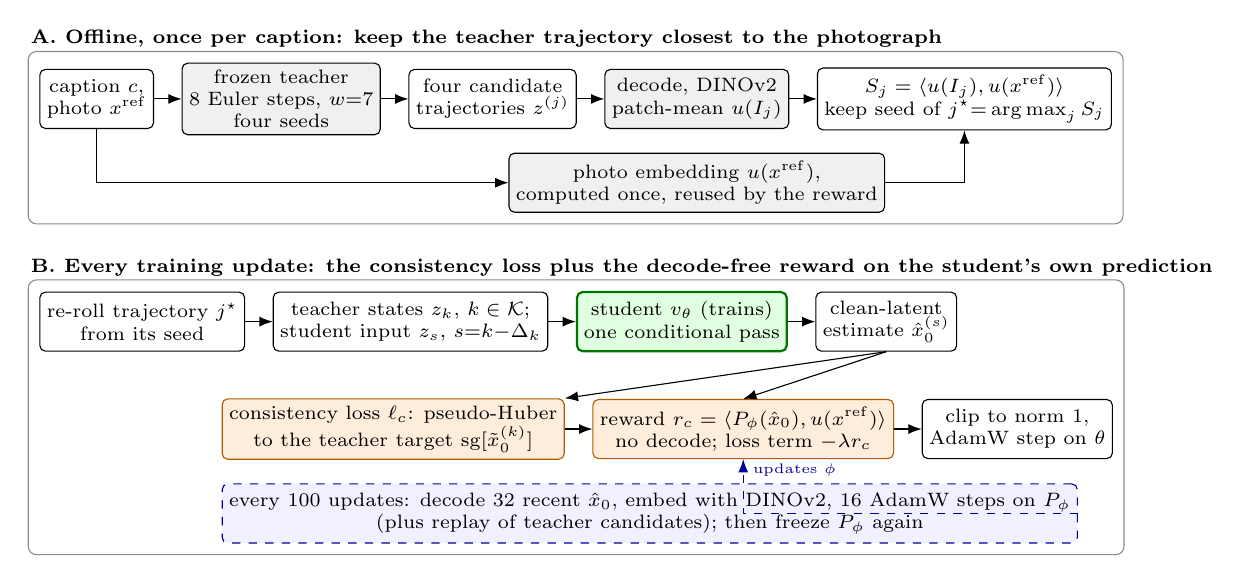
\begin{tikzpicture}[>=Latex, font=\scriptsize, node distance=3mm and 3.5mm,
  box/.style={draw, rounded corners=2pt, align=center, inner sep=2.5pt, minimum height=7.5mm, fill=white},
  frozen/.style={box, fill=black!6},
  train/.style={box, fill=green!12, draw=green!45!black, thick},
  loss/.style={box, fill=orange!14, draw=orange!70!black},
  refresh/.style={box, dashed, fill=blue!6, draw=blue!60!black},
  panel/.style={draw=black!45, rounded corners=3pt, inner sep=4pt},
  plabel/.style={font=\scriptsize\bfseries, anchor=south west, inner sep=1pt}]
% ---------------- panel A: offline selection
\node[box] (cap) {caption $c$,\\ photo $x^{\mathrm{ref}}$};
\node[frozen, right=of cap] (tea) {frozen teacher\\ 8 Euler steps, $w{=}7$\\ four seeds};
\node[box, right=of tea] (cand) {four candidate\\ trajectories $z^{(j)}$};
\node[frozen, right=of cand] (dec) {decode, DINOv2\\ patch-mean $u(I_j)$};
\node[box, right=of dec] (sc) {$S_j=\langle u(I_j),u(x^{\mathrm{ref}})\rangle$\\ keep seed of $j^\star{=}\argmaxop_j S_j$};
\node[frozen, below=of dec] (uref) {photo embedding $u(x^{\mathrm{ref}})$,\\ computed once, reused by the reward};
\draw[->] (cap) -- (tea); \draw[->] (tea) -- (cand); \draw[->] (cand) -- (dec); \draw[->] (dec) -- (sc);
\draw[->] (cap.south) |- (uref.west);
\draw[->] (uref.east) -| (sc.south);
\node[panel, fit=(cap)(tea)(cand)(dec)(sc)(uref)] (pA) {};
\node[plabel] at (pA.north west) {A.\ Offline, once per caption: keep the teacher trajectory closest to the photograph};
% ---------------- panel B: training update (two rows)
\node[box, anchor=north west] at ($(cap.west |- uref.south)+(0,-10mm)$) (roll) {re-roll trajectory $j^\star$\\ from its seed};
\node[box, right=of roll] (states) {teacher states $z_k$, $k\in\mathcal K$;\\ student input $z_s$, $s{=}k{-}\Delta_k$};
\node[train, right=of states] (stu) {student $v_\theta$ (trains)\\ one conditional pass};
\node[box, right=of stu] (xhat) {clean-latent\\ estimate $\hat x_0^{(s)}$};
\node[loss, below=6mm of xhat.south, anchor=north east, xshift=1mm] (rw) {reward $r_c=\langle P_\phi(\hat x_0),u(x^{\mathrm{ref}})\rangle$\\ no decode; loss term $-\lambda r_c$};
\node[loss, left=of rw] (lc) {consistency loss $\ell_c$: pseudo-Huber\\ to the teacher target $\sgop[\tilde x_0^{(k)}]$};
\node[box, right=of rw] (step) {clip to norm 1,\\ AdamW step on $\theta$};
\node[refresh, below=of lc.south west, anchor=north west, xshift=0mm] (ref) {every 100 updates: decode 32 recent $\hat x_0$, embed with DINOv2, 16 AdamW steps on $P_\phi$\\ (plus replay of teacher candidates); then freeze $P_\phi$ again};
\draw[->] (roll) -- (states); \draw[->] (states) -- (stu); \draw[->] (stu) -- (xhat);
\draw[->] (xhat.south) -- (rw.north); \draw[->] (xhat.south) -- (lc.north east);
\draw[->] (lc.east) -- (rw.west); \draw[->] (rw.east) -- (step.west);
\draw[->, dashed, blue!60!black] (ref.east) -| (rw.south) node[pos=0.9, right, font=\tiny]{updates $\phi$};
\node[panel, fit=(roll)(states)(stu)(xhat)(lc)(rw)(step)(ref)] (pB) {};
\node[plabel] at (pB.north west) {B.\ Every training update: the consistency loss plus the decode-free reward on the student's own prediction};
\end{tikzpicture}}
\caption{Overview. (A) Before training, each caption's four teacher trajectories are decoded, embedded with a
frozen DINOv2, scored against the caption's real photograph, and only the seed of the best one is kept.
(B) Each update re-rolls that trajectory, forms the student's clean-latent estimate from a noisier state,
and minimises the consistency loss minus a reward computed directly on the latent by the projector
$P_\phi$; no image is decoded on the training path. The dashed block refits $P_\phi$ every 100 updates.
Grey blocks are frozen; only the student (green) trains.}
\label{fig:overview}
\end{figure}

\subsection{Rectified-flow teacher and consistency distillation}
\label{sec:prelim}
The teacher is a rectified-flow model with frozen weights $\theta_T$, operating in the $D$-dimensional
latent space of a frozen VAE ($D{=}65{,}536$ at $512{\times}512$ pixels: a $16{\times}64{\times}64$
latent). A clean latent $x_0\in\mathbb R^D$ and Gaussian noise $\varepsilon\sim\mathcal N(0,I)$ define a
straight path $z_\sigma=(1-\sigma)x_0+\sigma\varepsilon$, $\sigma\in[0,1]$, and the network predicts the
velocity $v=\varepsilon-x_0$ conditioned on the caption $c$. Sampling is Euler integration on a $\sigma$
grid, $z_{k+1}=z_k+(\sigma_{k+1}-\sigma_k)\,v_\theta(z_k,\sigma_k,c)$, with classifier-free guidance
$v^{\mathrm{cfg}}=v_\theta(z,\sigma,\varnothing)+w\big(v_\theta(z,\sigma,c)-v_\theta(z,\sigma,\varnothing)\big)$
at $w=7$ for the teacher. The student $v_\theta$ is a full copy of the same transformer, initialised from
$\theta_T$, and is the only network that trains; the teacher, the text encoders and the VAE decoder
$\Dec$ stay frozen. There is no momentum target and no exponential moving average: every training
target below is a deterministic function of the frozen teacher.

\paragraph{Consistency loss.} Let $z_0,\dots,z_8$ be a teacher trajectory (8 Euler steps at $w{=}7$).
Training supervises a window of states $\mathcal K=\{3,4,5,6,7\}$ on the 8-step grid. For $k\in\mathcal K$,
the teacher's realised chord across its own step and the clean-latent estimate it implies are
\begin{equation}
\bar v_k=\frac{z_{k+1}-z_k}{\sigma_{k+1}-\sigma_k},\qquad
\tilde x_0^{(k)}=z_k-\sigma_k\,\bar v_k ,
\end{equation}
exact algebra for a straight path. The student is placed at a \emph{noisier} state than the one the target
was read from: for each $k$ we draw $\Delta_k\sim\mathcal U\{1,2,3\}$ afresh on every visit, set
$s=k-\Delta_k$, and the student forms its own clean-latent estimate with a single conditional forward
pass and no guidance,
\begin{equation}
\hat x_0^{(s)}=z_s-\sigma_s\,v_\theta(z_s,\sigma_s,c).
\end{equation}
The consistency loss is a pseudo-Huber distance in $x_0$-space, averaged over the window:
\begin{equation}
\ell_c(\theta)=\frac{1}{|\mathcal K|}\sum_{k\in\mathcal K}\rho\Big(\hat x_0^{(k-\Delta_k)}-\sgop\big[\tilde x_0^{(k)}\big]\Big),
\qquad \rho(u)=\sqrt{\lVert u\rVert_2^2+c_h^2}-c_h ,
\label{eq:cdloss}
\end{equation}
with $\sgop[\cdot]$ a stop-gradient and $c_h=0.00054\sqrt D\approx0.138$. This loss is what turns an
8-step teacher into a 4-step student; nothing below changes it. Because the student is trained with a
single conditional pass against $w{=}7$ teacher trajectories, guidance is absorbed into its prediction and
the student is sampled at $w{=}1$. What our method changes is \emph{which} trajectory the student is
trained on, and what, besides matching that trajectory, its own predictions are asked to do.

\subsection{Scored trajectory selection}
\label{sec:selection}
For every training caption $c$ with reference photograph $x^{\mathrm{ref}}$ (its COCO source image), we
draw $N=4$ candidate teacher trajectories from four seeds fixed by the caption index and score each against
the photograph. Candidate $j$ is an 8-step Euler rollout of the teacher at guidance $w=7$ from noise
$\varepsilon^{(j)}$; only the seed needs to be stored, since a candidate can be re-rolled exactly whenever it
is needed. Each candidate is decoded, $I_j=\Dec(z^{(j)}_8)$, and embedded with a frozen DINOv2-B vision
transformer: we drop the CLS token, mean-pool the $P{=}256$ patch tokens and $\ell_2$-normalise,
\begin{equation}
u(I)=\frac{\frac1P\sum_{p=1}^{P}h_p(I)}{\big\lVert\frac1P\sum_{p=1}^{P}h_p(I)\big\rVert},\qquad
S_j=\big\langle u(I_j),\,u(x^{\mathrm{ref}})\big\rangle ,\qquad
j^\star=\argmaxop_{j\in\{1,\dots,N\}}S_j .
\label{eq:score}
\end{equation}
$u(x^{\mathrm{ref}})$ is computed once per caption and reused by the reward below. Every subsequent visit
of caption $c$ trains only on trajectory $j^\star$. Selection is computed once, offline, before training
starts; no gradient flows through the scorer. The \naive{} baseline replaces $j^\star$ with a uniform draw
over $\{1,\dots,N\}$, stored so that every training seed sees the same draw: the two recipes see identical
candidate pools and differ only in which trajectory each caption trains on and in the reward term.

\subsection{A decode-free photographic reward}
\label{sec:reward}
Selection only changes which of the teacher's trajectories the student imitates; it never moves the
student's own predictions toward the photograph directly. The reward does, and it does so without decoding a
training image: a projector $P_\phi:\mathbb R^{16\times64\times64}\to\mathbb R^{768}$ maps a latent directly
into the DINOv2 patch-mean space of Equation~\ref{eq:score}, so a reward can be computed and differentiated on
the student's own latent prediction with no VAE decode and no DINOv2 forward pass on the training path.

\paragraph{Projector.} $P_\phi$ is a 10.7M-parameter convolutional encoder (five blocks, widths
$64,128,256,512,512$, the last four downsampling by 2, global-average-pooled) followed by a two-layer MLP
head ($512{\to}1024{\to}768$) and $\ell_2$-normalisation. It is pretrained once, offline, on 22,000
captions disjoint from every pool it later scores (Algorithm~\ref{alg:projpretrain} in
Appendix~\ref{app:proj}): for each cached candidate $z_j$ with true embedding $e_j=u(\Dec(z_j))$ and true
score $S_j$,
\begin{equation}
\mathcal L_{\mathrm{pre}}(\phi)=\mathrm{mean}_j\big[1-\langle P_\phi(z_j),e_j\rangle\big]\;+\;\mathrm{KL}\Big(\mathrm{softmax}(S/\tau)\,\big\|\,\mathrm{softmax}(\hat S/\tau)\Big),
\label{eq:projpretrain}
\end{equation}
where $\hat S_j=\langle P_\phi(z_j),u(x^{\mathrm{ref}})\rangle$ is the projector's own score and $\tau{=}0.04$; the first term matches the embedding, the second preserves the within-caption ranking
of the four candidates. On held-out captions the pretrained projector picks the same candidate as the
decoded scorer 49\% of the time (chance 25\%).

\paragraph{Reward.} On every update, the student's clean-latent estimates at the two least-noisy supervised
states are scored by $P_\phi$ directly:
\begin{equation}
r_c(\theta;\phi)=\frac12\sum_{i=1}^{2}\big\langle P_\phi\big(\hat x_0^{(s_i)}\big),\,u(x^{\mathrm{ref}})\big\rangle ,
\qquad
\mathcal L(\theta)=\mathbb E_c\big[\ell_c(\theta)\big]\;-\;\lambda\,\mathbb E_c\big[r_c(\theta;\phi)\big] .
\label{eq:objective}
\end{equation}
The gradient of $r_c$ flows through the frozen $P_\phi$ into $\theta$ only. We use $\lambda{=}80$, chosen so
that the raw reward gradient is about 20\% of the raw consistency gradient at initialisation (a
40-update probe measures a norm ratio of $0.22$); the sum is then clipped to global norm 1, so $\lambda$
sets the reward's share of the update direction rather than an absolute step size.

\paragraph{Periodic refresh.} $P_\phi$ was pretrained on the teacher's candidates, not on the evolving
predictions of a 4-step student, so its accuracy on what it actually scores during training is not
guaranteed. Every 100 updates $P_\phi$ is therefore unfrozen and refit to the true DINOv2 embeddings of the
student's 32 most recent predictions (decoded only for this refresh, not for the reward), together with a
replay term on a fresh batch of the original teacher-candidate data so it does not forget how to rank them:
\begin{equation}
\mathcal L_{\mathrm{refresh}}(\phi)=\mathrm{mean}\big[1-\langle P_\phi(\hat x_0),\,u(\Dec(\hat x_0))\rangle\big]\;+\;\mathcal L_{\mathrm{pre}}(\phi)\ \text{on a replay batch},
\label{eq:refresh}
\end{equation}
16 AdamW steps at learning rate $10^{-4}$ each time, after which $P_\phi$ is frozen again. Section~\ref{sec:results-abl}
compares this schedule with a frozen projector and with lighter refreshes.

\subsection{Training procedure and inference}
\label{sec:pseudocode}
Algorithm~\ref{alg:train} is one optimiser step. The two decodes in the whole pipeline happen outside the
gradient path: once per caption before training (selection, panel A of Figure~\ref{fig:overview}) and on
32 latents every 100 updates (the refresh). At inference the student is sampled with 4 Euler steps at
$w{=}1$: no guidance, no candidate generation, no projector. The trained student is a single network; nothing
about candidate pools, scorers, the projector or the reward survives into the deployed model.

\begin{algorithm}[t]
\caption{One training update of the student (repeat until the schedule ends)}
\label{alg:train}
\begin{algorithmic}[1]
\Require student $v_\theta$ (initialised from $\theta_T$); frozen teacher $v_T$, decoder $\Dec$ and DINOv2 $u(\cdot)$; pretrained projector $P_\phi$
\Statex \hspace{\algorithmicindent} per-caption seed $j^\star$ and embedding $u(x^{\mathrm{ref}})$ from selection; replay buffer of teacher candidates; $\mathcal K=\{3,\dots,7\}$; $\lambda{=}80$
\State pick a caption $c$; regenerate its selected trajectory $z_0,\dots,z_8$ from the stored seed \Comment{no decode}
\For{$k\in\mathcal K$} \Comment{five supervised noise levels, batched into one student forward pass}
  \State draw $\Delta_k\sim\mathcal U\{1,2,3\}$; $s\gets k-\Delta_k$
  \State $\hat x_0^{(s)}\gets z_s-\sigma_s\,v_\theta(z_s,\sigma_s,c)$;\quad $\tilde x_0^{(k)}\gets\sgop\big[z_k-\sigma_k\,(z_{k+1}-z_k)/(\sigma_{k+1}-\sigma_k)\big]$
\EndFor
\State $\ell_c\gets\frac{1}{|\mathcal K|}\sum_{k}\rho\big(\hat x_0^{(k-\Delta_k)}-\tilde x_0^{(k)}\big)$ \Comment{Equation~\ref{eq:cdloss}}
\State $r_c\gets\frac12\sum_{i=1}^{2}\langle P_\phi(\hat x_0^{(s_i)}),\,u(x^{\mathrm{ref}})\rangle$ for the two least-noisy $s$ \Comment{Equation~\ref{eq:objective}; no decode}
\State $g\gets\nabla_\theta[\ell_c-\lambda r_c]$; clip $g$ to global norm 1; AdamW step on $\theta$ \Comment{$\phi$ is not updated here}
\If{the update index is a multiple of 100} \Comment{refresh, Equation~\ref{eq:refresh}}
  \State decode the 32 most recent $\hat x_0$ and embed them with $u(\Dec(\cdot))$; sample a replay batch of teacher candidates
  \State 16 AdamW steps on $\phi$ (lr $10^{-4}$) minimising $\mathcal L_{\mathrm{refresh}}$; freeze $\phi$ again
\EndIf
\end{algorithmic}
\end{algorithm}

\section{Experimental Setup}
\label{sec:setup}

\paragraph{Data.} Training captions come from COCO \texttt{train2017}, each paired with the photograph it
was written for; the photograph is used only by the scorer and the reward and never enters the student's
input. All experiments below use a pool of 3,000 captions drawn once with a fixed seed. Evaluation uses a
separate, sealed pool built once with a fixed seed; fidelity references come from COCO \texttt{val2017}, so
no evaluation caption or photograph is seen in training.

\paragraph{Training configuration.} Both recipes use identical code, data order and hyperparameters
(Table~\ref{tab:hyper}); the only differences are the selected trajectory and the reward term. Every
reported student is the uniform weight average of its 2,000-, 4,000- and 6,000-update checkpoints, which
scores 0.015--0.02 CompBench above the raw final checkpoint for both recipes and removes most of the
checkpoint-to-checkpoint noise of a short schedule. Three training seeds
(0--2) are run per recipe; the two recipes share seeds, data order and $\Delta$ draws at equal seed, so
every comparison is seed-paired.

\begin{table}[t]
\centering
\caption{Training configuration (3k pool). The \naive{} baseline and our recipe share every entry.}
\label{tab:hyper}
\small
\begin{tabular}{l l}
\toprule
Captions / updates & 3,000 / 6,000 (2 passes), one caption per update, 1 GPU \\
Optimiser & AdamW, lr $10^{-5}$, 300 warm-up steps, weight decay 0, global grad-norm clip 1 \\
Precision & fp32 master weights, bf16 autocast, gradient checkpointing \\
Teacher / candidates & SD3.5-Medium, 8 Euler steps, $w{=}7$; $N{=}4$ candidates per caption \\
Consistency loss & pseudo-Huber in $x_0$-space, window $\mathcal K=\{3,\dots,7\}$, $\Delta_k\sim\mathcal U\{1,2,3\}$ \\
Reward (ours only) & $\lambda{=}80$ on the two least-noisy states; refresh every 100 updates, 16 steps, lr $10^{-4}$ \\
Reported weights & uniform average of the 2k / 4k / 6k checkpoints; 3 seeds per recipe \\
\bottomrule
\end{tabular}
\end{table}

\paragraph{Evaluation.} Alignment is measured with T2I-CompBench (8 categories: color, shape, texture,
2D-spatial, 3D-spatial, numeracy, non-spatial, complex; 2,398 sealed prompts, one image per prompt, the
official per-category scorers, reported as the unweighted mean of the eight categories) and GenEval2
(800 sealed prompts of 3--10 atomic conditions over object, count, attribute, position and verb skills; a
prompt scores the geometric mean of its atom scores, the official number is the mean over prompts,
$\times100$). Fidelity is measured with CMMD, precision, recall and FID against 5,000 held-out COCO
\texttt{val2017} photographs. Every arm and every seed is evaluated on exactly the same prompts and
initial noise, so per-prompt comparisons are like-for-like. All students are sampled with 4 Euler steps
at $w{=}1$.

\paragraph{Statistics.} Every contrast is a seed-paired difference (seed $s$ of ours minus seed $s$ of
\naive{}), reported as mean $\pm$ standard deviation over the three seeds with the paired $t$-test $p$-value.
Three seeds is a small sample: $p$-values below 0.05 are reported as resolved, everything else as
unresolved, and every table shows the per-seed spread so the reader can judge.

\section{Results}
\label{sec:results}

\subsection{Main result: scored distillation with the projector reward beats \naive{}}
\label{sec:results-main}
Table~\ref{tab:main} and Figure~\ref{fig:arms} give the headline comparison. On T2I-CompBench our student
scores $0.4887\pm0.0025$ against $0.4738\pm0.0017$ for \naive{}: a seed-paired gain of
$+0.0149\pm0.0017$ ($p{=}0.004$), positive on every seed (per-seed $+0.0146$, $+0.0134$, $+0.0167$). On
GenEval2 it scores $23.5$ against $22.5$ ($+1.00\pm0.91$), positive on two seeds and flat on the third,
not resolved at three seeds. For scale, the same 4-step budget without distillation (the base model at 4
steps, $w{=}7$) reaches only $0.256$ CompBench, and the 28-step guided teacher reaches $0.505$: the
student closes most of the gap between a 4-step and a 28-step sampler, and our recipe recovers about half
of the remaining distance to the teacher over \naive{}.

\begin{table}[t]
\centering
\caption{Alignment on the sealed evaluation pools. Both students: 3k captions, three training seeds,
averaged checkpoints, one image per prompt, 4 steps, $w{=}1$. $\Delta$ is the seed-paired difference to
\naive{} (mean $\pm$ sd over seeds, paired $t$-test $p$). Reference rows are single deterministic runs of
the undistilled model.}
\label{tab:main}
\fitbox{\begin{tabular}{l c c c c}
\toprule
Model & CompBench & $\Delta$ vs.\ naive ($p$) & GenEval2 ($\times100$) & $\Delta$ vs.\ naive ($p$) \\
\midrule
Naive CD (random trajectory, no reward) & $0.4738\pm0.0017$ & -- & $22.53\pm0.95$ & -- \\
\textbf{Ours} (scored trajectory + projector reward) & $\mathbf{0.4887}\pm0.0025$ & $+0.0149\pm0.0017$ (0.004) & $\mathbf{23.54}\pm1.56$ & $+1.00\pm0.91$ (0.20) \\
\midrule
Base model, 4 steps, $w{=}7$ (no distillation) & $0.2557$ & -- & $7.32$ & -- \\
Teacher, 8 steps, $w{=}7$ (the distillation source) & $0.4544$ & -- & $17.58$ & -- \\
Teacher, 28 steps, $w{=}7$ & $0.5053$ & -- & $17.05$ & -- \\
\bottomrule
\end{tabular}}
\end{table}

\begin{figure}[t]
\centering
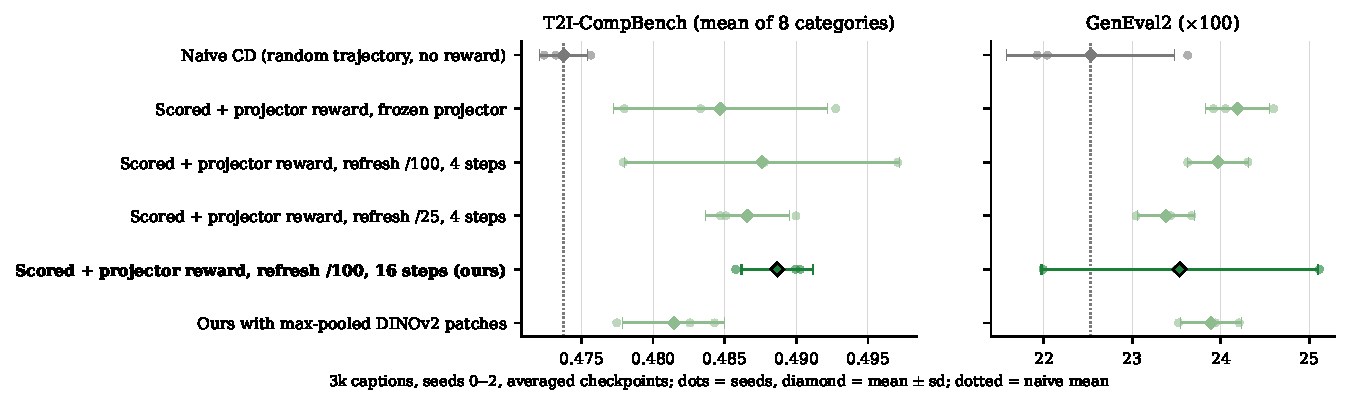
\includegraphics[width=\textwidth]{arms_3k.pdf}
\caption{Every recipe of this paper on the two alignment benchmarks (3k captions, seeds 0--2, averaged
checkpoints). Dots are training seeds, diamonds the mean $\pm$ sd, the dotted line the \naive{} mean. Our
recipe (bold) is the only one whose three seeds all sit clear of the \naive{} spread on CompBench.}
\label{fig:arms}
\end{figure}

\paragraph{Where the gain is.} Figure~\ref{fig:cat} and Table~\ref{tab:cat} split the CompBench gain by
category. The improvement is broad rather than concentrated: seven of the eight categories move in our
favour on the seed mean, and three are resolved at three seeds, colour ($+0.021$, $p{=}0.017$), shape
($+0.019$, $p{<}0.001$) and the long-caption ``complex'' category ($+0.012$, $p{=}0.010$). The largest
mean gain is on 2D-spatial relations ($+0.032$) but with a wide seed spread ($p{=}0.09$); texture
($+0.017$) and numeracy ($+0.009$) are also positive but unresolved. Non-spatial prompts, scored by
CLIPScore, do not move for either recipe.

\begin{figure}[t]
\centering
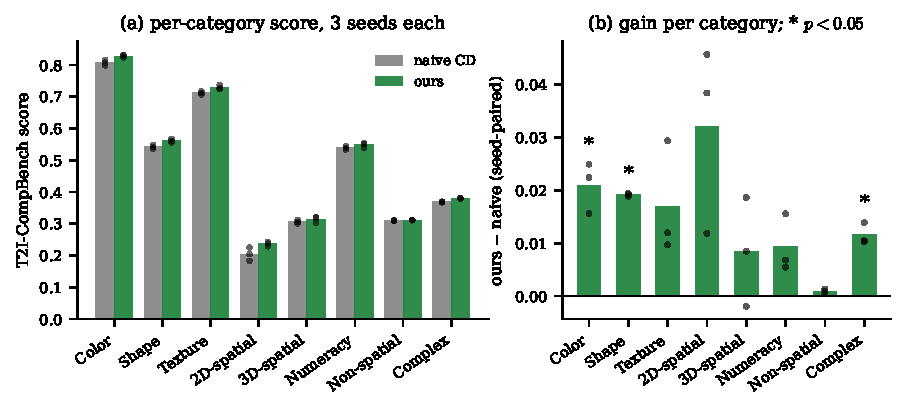
\includegraphics[width=\textwidth]{category_gains.pdf}
\caption{CompBench by category. (a) Per-category scores of \naive{} and ours, dots are seeds. (b)
Seed-paired gain of ours over \naive{}; dots are the three per-seed differences, stars mark $p<0.05$.}
\label{fig:cat}
\end{figure}

\begin{table}[t]
\centering
\caption{CompBench by category, 3k pool, seeds 0--2, averaged checkpoints, one image per prompt.}
\label{tab:cat}
\fitbox{\begin{tabular}{l c c c}
\toprule
Category & Naive CD & Ours & Ours $-$ naive ($p$) \\
\midrule
Color & $0.8075\pm0.0088$ & $0.8284\pm0.0044$ & $+0.0210\pm0.0048$ (0.02) \\
Shape & $0.5421\pm0.0060$ & $0.5613\pm0.0058$ & $+0.0192\pm0.0003$ ($<0.001$) \\
Texture & $0.7123\pm0.0049$ & $0.7294\pm0.0066$ & $+0.0170\pm0.0108$ (0.11) \\
2D-spatial & $0.2044\pm0.0212$ & $0.2364\pm0.0070$ & $+0.0320\pm0.0178$ (0.09) \\
3D-spatial & $0.3058\pm0.0053$ & $0.3142\pm0.0096$ & $+0.0084\pm0.0103$ (0.29) \\
Numeracy & $0.5391\pm0.0052$ & $0.5484\pm0.0078$ & $+0.0093\pm0.0055$ (0.10) \\
Non-spatial & $0.3103\pm0.0006$ & $0.3112\pm0.0002$ & $+0.0009\pm0.0004$ (0.07) \\
Complex & $0.3685\pm0.0014$ & $0.3801\pm0.0011$ & $+0.0116\pm0.0020$ (0.01) \\
\midrule
\textbf{Mean} & $0.4738\pm0.0017$ & $0.4887\pm0.0025$ & $+0.0149\pm0.0017$ (0.004) \\
\bottomrule
\end{tabular}}
\end{table}

\paragraph{GenEval2 by skill and prompt complexity.} Appendix~\ref{app:geneval} breaks GenEval2 down.
The share of prompts on which at least one atom is entirely wrong (``collapsed'', geometric mean below
$0.05$) falls from $36.6\%$ to $33.7\%$ ($-3.0\pm1.4$, $p{=}0.07$), the position skill gains the most
($+3.7\pm1.7$ per atom, $p{=}0.06$) and attribute binding gains $+1.8$; object presence and counting are
unchanged, and the verb skill, the weakest for every 4-step model, moves within noise ($-1.5\pm3.4$).

\subsection{Projector-reward ablations}
\label{sec:results-abl}
Table~\ref{tab:abl} varies only the reward, keeping scored selection and everything else fixed, and
compares every variant with \naive{}. Three findings. (i) Every variant beats \naive{} on the seed mean, but
only the refreshed projector with 16 steps per refresh (ours) does so with a tight, resolved margin
($+0.0149\pm0.0017$); the frozen projector ($+0.0109\pm0.0075$) and the default 4-step refresh
($+0.0138\pm0.0093$) reach a similar mean at three times the seed spread, and refreshing four times as
often with 4 steps ($+0.0128\pm0.0037$, $p{=}0.03$) does not match 16 steps at the original cadence. The
refresh therefore mainly buys \emph{consistency across seeds}, which is what makes the gain resolvable.
(ii) The refresh does what it is meant to: during training the projector score of the student's own
predictions rises by $0.04$--$0.07$ in every seed while the true DINOv2 score of the same decoded latents
stays flat ($-0.03$ to $0.00$), and the within-batch correlation between the two is $0.42$ over the
second half of training with the refresh against $0.36$ with a frozen projector; the projector tracks the
ranking of the student's predictions but not their absolute photographic similarity, which is why we
read it as a regulariser that keeps the student near the photograph-like candidates it was selected on,
rather than as a faithful reward. (iii) The DINOv2 pooling matters: replacing
mean pooling of the patch tokens by max pooling, in both the selection score and the reward, halves the
gain ($+0.0077\pm0.0023$). Max pooling compresses the within-caption spread of candidate scores tenfold
(standard deviation $0.007$ against $0.069$), so at the same $\lambda$ the reward gradient is ten times
smaller (probe ratio $0.022$ against $0.22$); the selection it induces agrees with mean pooling on only
60\% of captions.

\begin{table}[t]
\centering
\caption{Reward ablations, 3k pool, seeds 0--2, averaged checkpoints. Every row except the first uses
scored trajectory selection with the projector reward ($\lambda{=}80$) and differs only in how the
projector is refreshed (or, in the last row, in the DINOv2 pooling used for both selection and reward).
$\Delta$ is seed-paired against \naive{}. CMMD (lower is better) is the seed mean on 5,000 COCO val2017 captions.}
\label{tab:abl}
\fitbox{\begin{tabular}{l c c c c c}
\toprule
Reward variant & CompBench & $\Delta$ vs.\ naive ($p$) & GenEval2 & $\Delta$ vs.\ naive ($p$) & CMMD$\downarrow$ \\
\midrule
Naive CD (no selection, no reward) & $0.4738\pm0.0017$ & -- & $22.5\pm0.9$ & -- & $0.837$ \\
Projector frozen & $0.4847\pm0.0075$ & $+0.0109\pm0.0075$ (0.13) & $24.2\pm0.4$ & $+1.66\pm0.60$ (0.04) & $0.810$ \\
Refresh every 100 updates, 4 steps & $0.4876\pm0.0096$ & $+0.0138\pm0.0093$ (0.12) & $24.0\pm0.3$ & $+1.44\pm1.02$ (0.14) & $0.843$ \\
Refresh every 25 updates, 4 steps & $0.4866\pm0.0029$ & $+0.0128\pm0.0037$ (0.03) & $23.4\pm0.3$ & $+0.85\pm0.71$ (0.17) & $0.833$ \\
\textbf{Refresh every 100 updates, 16 steps (ours)} & $0.4887\pm0.0025$ & $+0.0149\pm0.0017$ (0.004) & $23.5\pm1.6$ & $+1.00\pm0.91$ (0.20) & $0.817$ \\
Ours, max-pooled DINOv2 patches & $0.4814\pm0.0036$ & $+0.0077\pm0.0023$ (0.03) & $23.9\pm0.3$ & $+1.36\pm0.99$ (0.14) & -- \\
\bottomrule
\end{tabular}}
\end{table}

\subsection{Fidelity}
\label{sec:results-fid}
Alignment gains that are bought with image quality are not gains, so Tables~\ref{tab:fid3k}
and~\ref{tab:fid118k} report fidelity against real photographs at both scales. At 3k the picture is
mixed and small: our student is slightly closer to the real distribution on CMMD ($0.817$ against
$0.837$; $-0.020\pm0.026$, unresolved), its recall is higher on every seed ($+0.013\pm0.003$, $p{=}0.02$),
precision is unchanged, and FID is marginally worse ($+0.47\pm0.14$ on a base of $30$; $p{=}0.03$). At
118k the picture is not mixed: our student is worse than \naive{} on every measure and on every seed --
CMMD $+0.037\pm0.006$ ($p{=}0.008$), precision $-0.014\pm0.005$ ($p{=}0.04$), recall $-0.011\pm0.003$
($p{=}0.02$), FID $+0.92\pm0.13$ ($p{=}0.007$). The alignment gain at scale is therefore paid for with a
measurable loss of photographic fidelity. This is consistent with the training-time diagnostic of
Section~\ref{sec:results-abl}: the reward moves the student toward what the projector scores as
photograph-like, and over a long schedule that is not the same as the real photograph distribution. We
report it as a limitation of the projector reward rather than explain it away; a reward that tracks the
true score more faithfully (Section~\ref{sec:results-abl}) is the obvious remedy.

\begin{table}[t]
\centering
\caption{Fidelity on 5,000 COCO val2017 captions, 3k pool, seeds 0--2, averaged checkpoints, 4 steps,
$w{=}1$. Contrasts are seed-paired (mean $\pm$ sd, paired $t$-test $p$).}
\label{tab:fid3k}
\fitbox{\begin{tabular}{l c c c c}
\toprule
 & CMMD $\downarrow$ & Precision $\uparrow$ & Recall $\uparrow$ & FID $\downarrow$ \\
\midrule
Naive CD & $0.837\pm0.042$ & $0.479\pm0.025$ & $0.054\pm0.003$ & $30.42\pm0.17$ \\
\textbf{Ours} & $0.817\pm0.025$ & $0.474\pm0.013$ & $0.067\pm0.001$ & $30.89\pm0.22$ \\
\midrule
Ours $-$ naive (seed-paired, $p$) & $-0.020\pm0.026$ (0.32) & $-0.005\pm0.014$ (0.60) & $+0.013\pm0.003$ (0.02) & $+0.47\pm0.14$ (0.03) \\
\bottomrule
\end{tabular}}
\end{table}

\begin{table}[t]
\centering
\caption{Fidelity at 118k on the same 5,000 COCO val2017 captions, per seed (0 / 1 / 2), last-five-checkpoint
averages, 4 steps, $w{=}1$. Contrasts are seed-paired (mean $\pm$ sd, paired $t$-test $p$).}
\label{tab:fid118k}
\fitbox{\begin{tabular}{l c c c c}
\toprule
118k, seeds 0 / 1 / 2, last-5 average & CMMD $\downarrow$ & Precision $\uparrow$ & Recall $\uparrow$ & FID $\downarrow$ \\
\midrule
Naive CD & 0.84/0.84/0.83 & 0.485/0.489/0.503 & 0.059/0.066/0.062 & 31.08/30.97/31.44 \\
\textbf{Ours} & 0.88/0.88/0.86 & 0.477/0.472/0.487 & 0.047/0.053/0.054 & 31.85/31.95/32.46 \\
\midrule
Ours $-$ naive (seed-paired, $p$) & $+0.037\pm0.006$ (0.008) & $-0.014\pm0.005$ (0.04) & $-0.011\pm0.003$ (0.02) & $+0.92\pm0.13$ (0.007) \\
\bottomrule
\end{tabular}}
\end{table}

\subsection{Qualitative results}
\label{sec:results-qual}
Figures~\ref{fig:qual-cb} and~\ref{fig:qual-ge} compare the two students prompt by prompt. Every column of
a row starts from the same initial noise, so differences down a row are due to the model, not the draw. We
also show the undistilled base model at the same 4-step budget, which is why distillation is needed at
all, and the 28-step guided teacher as the ceiling. The rows are curated: for each CompBench category we
ranked prompts by the ours-minus-\naive{} margin averaged over the three seeds and, among the top eight,
kept one whose difference is visible in the image rather than only in the evaluator's score;
Appendix~\ref{app:qual} shows an uncurated random draw and the prompts on which \naive{} scores higher.
The pattern in the curated rows is consistent: the second object of a two-object prompt that \naive{}
drops appears (the black whiskers, the laptop next to the bag, the cameras with the horses, the silver
car beside the truck), a fluffy or metallic material that was named becomes visible, and object counts
and spatial relations that \naive{} gets approximately right become exact (three turtles, five cats on
the suitcase, three monkeys on the clock, the bagel to the right of the kangaroos). In the uncurated rows
the two students are visually near-identical: the gain is concentrated on a minority of prompts, which is
also what the per-prompt statistics say (on 21--30\% of colour, shape and texture prompts our student
scores at least $0.05$ higher, on 11--16\% \naive{} does).

Figure~\ref{fig:qual-spatial} shows two 2D-spatial prompts on which our student places the objects as
asked at 4, 8 and 28 sampling steps alike while the guided 28-step teacher does not: a distilled few-step
student is not, skill by skill, a strictly degraded copy of its many-step teacher.

\begin{figure}[p]
\centering

\includegraphics[width=\textwidth,height=0.9\textheight,keepaspectratio]{qual_compbench.jpg}
\caption{T2I-CompBench, one curated prompt per category (colour, shape, texture, 2D-spatial, 3D-spatial,
numeracy, complex). Columns share the initial noise. Scores under the images are the official
per-category evaluator's score for that image. Base model: SD3.5-Medium sampled at the student's 4-step
budget with guidance $w{=}7$, no distillation.}
\label{fig:qual-cb}
\end{figure}

\begin{figure}[p]
\centering

\includegraphics[width=\textwidth,height=0.55\textheight,keepaspectratio]{qual_geneval2.jpg}
\caption{GenEval2, curated prompts on counting, relations and attribute binding. Scores under the images
are the prompt's geometric mean over its atoms. Columns share the initial noise.}
\label{fig:qual-ge}
\vspace{5mm}

\includegraphics[width=0.9\textwidth,height=0.26\textheight,keepaspectratio]{qual_spatial_paper.pdf}
\caption{Two T2I-CompBench 2D-spatial prompts, identical initial noise per prompt. Our student (no
guidance) places both named objects in the requested relation at 4, 8 and 28 sampling steps alike; the
frozen teacher with guidance ($w{=}7$) does not at 28 steps. Green borders: the requested relation is
satisfied; red: it is not. Automatic 2D-spatial scores (computed for the 4-step student and the teacher
only): 0.92 vs.\ 0.00 (top), 0.78 vs.\ 0.00 (bottom).}
\label{fig:qual-spatial}
\end{figure}

\subsection{Scaling to 118,000 captions}
\label{sec:results-scale}
To test whether the recipe survives a forty-fold larger caption pool, both recipes were trained on the
complete COCO \texttt{train2017} caption set (113,948 captions, two passes, 56,974 updates on 4 GPUs
with one caption per GPU per update, learning rate $2\times10^{-5}$, 1,000 warm-up steps, three seeds
each). Under this long schedule single checkpoints oscillate by up to 0.03 CompBench from one save to
the next (Table~\ref{tab:scale}, last row), so, as for the 3k runs, the reported student of each run is
the uniform weight average of its last five checkpoints (40k, 45k, 50k, 55k and final).

Table~\ref{tab:scale} gives the result. Our recipe scores $0.4810\pm0.0050$ CompBench against
$0.4668\pm0.0036$ for \naive{}: $+0.0142\pm0.0085$ seed-paired ($+0.019$, $+0.004$, $+0.019$ on the
three seeds), the same size as the 3k gain. With three seeds the seed-level test is not resolved
($p{=}0.10$), but the prompt-level test on seed-averaged per-prompt scores over the 2,398 prompts is
($p{=}4\times10^{-9}$). GenEval2 moves from $20.3$ to $21.7$ ($+1.37\pm1.28$; prompt-level $p{=}0.016$), and
the share of collapsed prompts falls from $44\%$ to $41\%$. Table~\ref{tab:scale_cat} shows the gain is
again broad: colour ($+0.021$, $p{=}0.04$), numeracy ($+0.019$), 3D-spatial ($+0.019$), shape ($+0.018$),
texture ($+0.018$) and 2D-spatial ($+0.014$) all move in our favour on the seed mean, with only the
CLIP-scored non-spatial category flat. What scale does \emph{not} buy is absolute quality: the 118k
students are no better than their 3k counterparts (\naive{} $0.467$ vs.\ $0.474$; ours $0.481$ vs.\
$0.489$) despite ten times the updates, and their consistency loss ends at the same level. We return to
this in Section~\ref{sec:results-schedule}.

\begin{table}[t]
\centering
\caption{118k captions, 56,974 updates, three training seeds, last-five-checkpoint averages, 4 steps,
$w{=}1$. Seed-paired contrasts as in Table~\ref{tab:main}; the prompt-level $p$ is a paired $t$-test over
the 2,398 CompBench (800 GenEval2) prompts after averaging each prompt's score over the three seeds.}
\label{tab:scale}
\fitbox{\begin{tabular}{l c c c c c c}
\toprule
 & \multicolumn{3}{c}{CompBench} & \multicolumn{3}{c}{GenEval2 ($\times100$)} \\
\cmidrule(lr){2-4}\cmidrule(lr){5-7}
Recipe (118k captions, 3 seeds, last-5 average) & mean $\pm$ sd & $\Delta$ vs.\ naive, seed-paired ($p$) & prompt-level $p$ & mean $\pm$ sd & $\Delta$ vs.\ naive ($p$) & prompt-level $p$ \\
\midrule
Naive CD (random trajectory, no reward) & $0.4668\pm0.0036$ & -- & -- & $20.29\pm0.48$ & -- & -- \\
\textbf{Ours} (scored trajectory + projector reward) & $\mathbf{0.4810}\pm0.0050$ & $+0.0142\pm0.0085$ (0.10) & $<0.001$ & $\mathbf{21.66}\pm1.13$ & $+1.37\pm1.28$ (0.21) & 0.02 \\
\midrule
\multicolumn{7}{l}{\footnotesize Raw final checkpoints (before averaging), CompBench per seed: naive 0.4573 / 0.4570 / 0.4591; ours 0.4584 / 0.4514 / 0.4718} \\
\bottomrule
\end{tabular}}
\end{table}

\begin{table}[t]
\centering
\caption{CompBench by category at 118k, three seeds, last-five-checkpoint averages, one image per prompt.}
\label{tab:scale_cat}
\fitbox{\begin{tabular}{l c c c}
\toprule
Category (118k, 3 seeds, last-5 average) & Naive CD & Ours & Ours $-$ naive ($p$) \\
\midrule
Color & $0.7755\pm0.0044$ & $0.7965\pm0.0029$ & $+0.0209\pm0.0071$ (0.04) \\
Shape & $0.5338\pm0.0066$ & $0.5515\pm0.0102$ & $+0.0177\pm0.0168$ (0.21) \\
Texture & $0.7051\pm0.0063$ & $0.7226\pm0.0041$ & $+0.0175\pm0.0099$ (0.09) \\
2D-spatial & $0.1971\pm0.0086$ & $0.2109\pm0.0113$ & $+0.0138\pm0.0199$ (0.35) \\
3D-spatial & $0.2999\pm0.0041$ & $0.3190\pm0.0068$ & $+0.0190\pm0.0109$ (0.09) \\
Numeracy & $0.5483\pm0.0029$ & $0.5673\pm0.0061$ & $+0.0189\pm0.0084$ (0.06) \\
Non-spatial & $0.3141\pm0.0006$ & $0.3126\pm0.0010$ & $-0.0014\pm0.0008$ (0.10) \\
Complex & $0.3606\pm0.0030$ & $0.3677\pm0.0023$ & $+0.0071\pm0.0042$ (0.10) \\
\midrule
\textbf{Mean} & $0.4668\pm0.0036$ & $0.4810\pm0.0050$ & $+0.0142\pm0.0085$ (0.10) \\
\bottomrule
\end{tabular}}
\end{table}

\subsection{Optimisation, not data, limits the 4-step student}
\label{sec:results-schedule}
The 118k runs expose a property of the training recipe rather than of the method: the consistency loss
plateaus early and neither more captions nor more updates lower it. Both configurations use a linear
warm-up followed by a \emph{constant} learning rate, and the pre-clip gradient norm (130--900) exceeds
the clipping threshold of 1 on every update, so every update is a fixed-size normalised step and the
weights random-walk on a plateau, which is also why single checkpoints oscillate and why averaging is
needed. Under this schedule the loss falls by the same 7\% over the first 6,000 updates at 3k and over
57,000 updates at 118k, the per-noise-level losses end at the same values at both scales, and the
noisiest supervised state ($k{=}3$) carries a third of the loss and never improves.

We therefore re-ran both recipes on the 3k pool with a converged schedule -- cosine decay to zero,
an effective batch of 16 captions (4 GPUs $\times$ 4 accumulated), peak learning rate $10^{-5}$ and the
supervised window narrowed to $\mathcal K=\{4,5,6,7\}$ -- for 3,000 updates (one seed). The
optimisation problem disappears: raw final and averaged checkpoints agree to $0.002$, and \naive{} alone
rises to $0.486$ CompBench, above its old averaged score and above every old-schedule 118k student. On
this converged baseline our recipe scores $0.488$: the edge shrinks from $+0.015$ to $+0.002$--$0.003$,
inside single-seed noise, with ours still ahead on shape, numeracy and complex prompts and behind on
2D-spatial ones. The honest reading is that scored selection with the projector reward mostly
compensates for weak optimisation; it is not additive with a well-converged schedule at this scale. The
same converged schedule at 118k (two passes, 14,244 updates of 16 captions, one seed) gives \naive{}
$0.4747$ and ours $0.4818$ on the last-five average ($0.4744$ and $0.4780$ on the raw final checkpoints;
GenEval2 $21.9$ and $22.3$): a $+0.007$ edge for our recipe, between the old-schedule gain and the 3k
converged result, and, notably, both 118k students remain below their 3k counterparts trained for
sixteen passes -- at this compute the distillation is limited by optimisation and by the number of
passes over the selected trajectories, not by the number of distinct captions.

\subsection{Additional ablations}
\label{sec:appendix-titles}
The following one-factor ablations were run on the 3k pool with the same protocol and are reported in the
appendix; only their titles are given here.
\begin{itemize}
\item Selection rule: hard selection of the best candidate vs.\ Boltzmann-weighted vs.\ sampled vs.\ uniform candidate weighting.
\item Projector refresh schedule: frozen vs.\ every 100 updates at 4 or 16 steps vs.\ every 25 updates (Table~\ref{tab:abl}).
\item DINOv2 patch pooling: mean vs.\ max, for selection and reward (Table~\ref{tab:abl}).
\item Consistency-target horizon: 1-step estimate vs.\ a 2-step chord vs.\ the trajectory endpoint.
\item Training objective: $x_0$ regression vs.\ segment-velocity imitation.
\item Teacher quality: candidate generation and training with a 16-step and a 28-step teacher.
\item Regression onto the reference photograph as a second training target.
\item An evolving (exponential-moving-average) teacher in place of the frozen teacher.
\item Inference step count: sampling the 4-step student at 2, 8, 16 and 28 steps.
\end{itemize}

\appendix
\section{Projector pretraining}
\label{app:proj}
\begin{algorithm}[h]
\caption{Pretrain the projector $P_\phi$ (once, before any student training)}
\label{alg:projpretrain}
\begin{algorithmic}[1]
\Require 22,000 captions' cached candidates ($z_j$, true embedding $e_j=u(\Dec(z_j))$, true score $S_j$), disjoint from any pool $P_\phi$ will later score; $\tau{=}0.04$
\State initialise $P_\phi$: 5-block conv encoder (widths 64,128,256,512,512) + MLP head ($512{\to}1024{\to}768$) + $\ell_2$-normalise
\For{30 epochs, batches of 32 captions (128 candidates)}
  \State $\hat e_j\gets P_\phi(z_j)$;\quad $\hat S_j\gets\langle\hat e_j,u(x^{\mathrm{ref}})\rangle$
  \State $\mathcal L_{\mathrm{pre}}\gets\mathrm{mean}_j[1-\langle\hat e_j,e_j\rangle]+\mathrm{KL}\big(\mathrm{softmax}(S/\tau)\,\|\,\mathrm{softmax}(\hat S/\tau)\big)$ \Comment{Equation~\ref{eq:projpretrain}}
  \State AdamW step on $\phi$ (one-cycle schedule, peak lr $3{\times}10^{-4}$)
\EndFor
\State keep the epoch with the lowest selection regret on 2,000 validation captions; freeze $\phi$
\end{algorithmic}
\end{algorithm}
The 27,000 captions used here (22,000 training, 2,000 validation, 3,000 test) are disjoint from the 3k
training pool's captions only in their role: the 3,000 test captions \emph{are} the training pool, on
which the projector is evaluated but never trained. On them the pretrained projector agrees with the
decoded scorer's choice on 49\% of captions and its selection regret, the decoded score of the decoded
argmax minus that of the projector's argmax, is $0.029$.

\section{GenEval2 breakdown}
\label{app:geneval}
\begin{table}[h]
\centering
\caption{GenEval2 by skill and by prompt complexity, 3k pool, seeds 0--2, averaged checkpoints. Overall
is the official score (each prompt's geometric mean over its atoms, averaged over prompts); collapsed is
the share of prompts with a geometric mean below $0.05$, i.e.\ at least one atom entirely wrong. Skill
rows are the mean score of the atoms tagged with that skill; atom-count rows are the mean score of the
atoms of prompts with that many atoms (100 prompts per count).}
\label{tab:geneval}
\fitbox{\begin{tabular}{l c c c}
\toprule
GenEval2 measure ($\times100$), 3k, seeds 0--2 & Naive CD & Ours & Ours $-$ naive ($p$) \\
\midrule
Overall (official; per-prompt geometric mean) & $22.5\pm0.9$ & $23.5\pm1.6$ & $+1.0\pm0.9$ (0.20) \\
Collapsed prompts (\%; score $<0.05$) & $36.6\pm3.4$ & $33.7\pm2.1$ & $-3.0\pm1.4$ (0.07) \\
\midrule
Skill: object (per atom) & $84.2\pm1.8$ & $84.1\pm0.8$ & $-0.0\pm1.2$ (0.95) \\
Skill: count (per atom) & $36.2\pm0.9$ & $36.5\pm1.1$ & $+0.3\pm1.3$ (0.74) \\
Skill: attribute (per atom) & $70.8\pm1.1$ & $72.5\pm1.4$ & $+1.8\pm1.7$ (0.22) \\
Skill: position (per atom) & $47.4\pm3.7$ & $51.1\pm2.0$ & $+3.7\pm1.7$ (0.06) \\
Skill: verb (per atom) & $26.1\pm3.9$ & $24.6\pm1.0$ & $-1.5\pm3.4$ (0.53) \\
\midrule
Atoms $=3$ (per atom) & $73.7\pm0.6$ & $73.1\pm1.1$ & $-0.6\pm1.5$ (0.53) \\
Atoms $=4$ (per atom) & $70.2\pm1.5$ & $72.0\pm1.2$ & $+1.8\pm0.6$ (0.04) \\
Atoms $=5$ (per atom) & $65.5\pm0.9$ & $66.8\pm1.8$ & $+1.3\pm1.7$ (0.32) \\
Atoms $=6$ (per atom) & $65.2\pm0.5$ & $65.0\pm1.9$ & $-0.1\pm1.5$ (0.91) \\
Atoms $=7$ (per atom) & $61.6\pm0.9$ & $60.9\pm1.0$ & $-0.8\pm0.2$ (0.01) \\
Atoms $=8$ (per atom) & $57.4\pm2.1$ & $58.1\pm1.6$ & $+0.7\pm2.7$ (0.70) \\
Atoms $=9$ (per atom) & $55.4\pm1.9$ & $58.3\pm1.2$ & $+2.9\pm1.6$ (0.09) \\
Atoms $=10$ (per atom) & $50.6\pm2.0$ & $51.3\pm1.6$ & $+0.7\pm3.0$ (0.73) \\
\bottomrule
\end{tabular}}
\end{table}

\section{Additional qualitative results}
\label{app:qual}
Figures~\ref{fig:unc-cb} and~\ref{fig:unc-ge} show an uncurated random draw of prompts (a fixed random
seed, no selection on scores). Figures~\ref{fig:reg-cb} and~\ref{fig:reg-ge} show the prompts with the
largest \naive{}-over-ours margin. On the two CompBench prompts the images are nearly identical and the
score difference comes from the automatic evaluator (the pig's snout overlapping the clock face defeats
the object detector; the bracelet-and-knife pair is scored by a VQA model that answers differently on
near-identical crops); this evaluator sensitivity is the main source of per-prompt noise in both
benchmarks. On the two GenEval2 prompts our student makes a genuine counting error, drawing one object too
many (eight or nine dogs, five backpacks), which the geometric-mean scoring punishes with a score near
zero.

\begin{figure}[!htb]
\centering
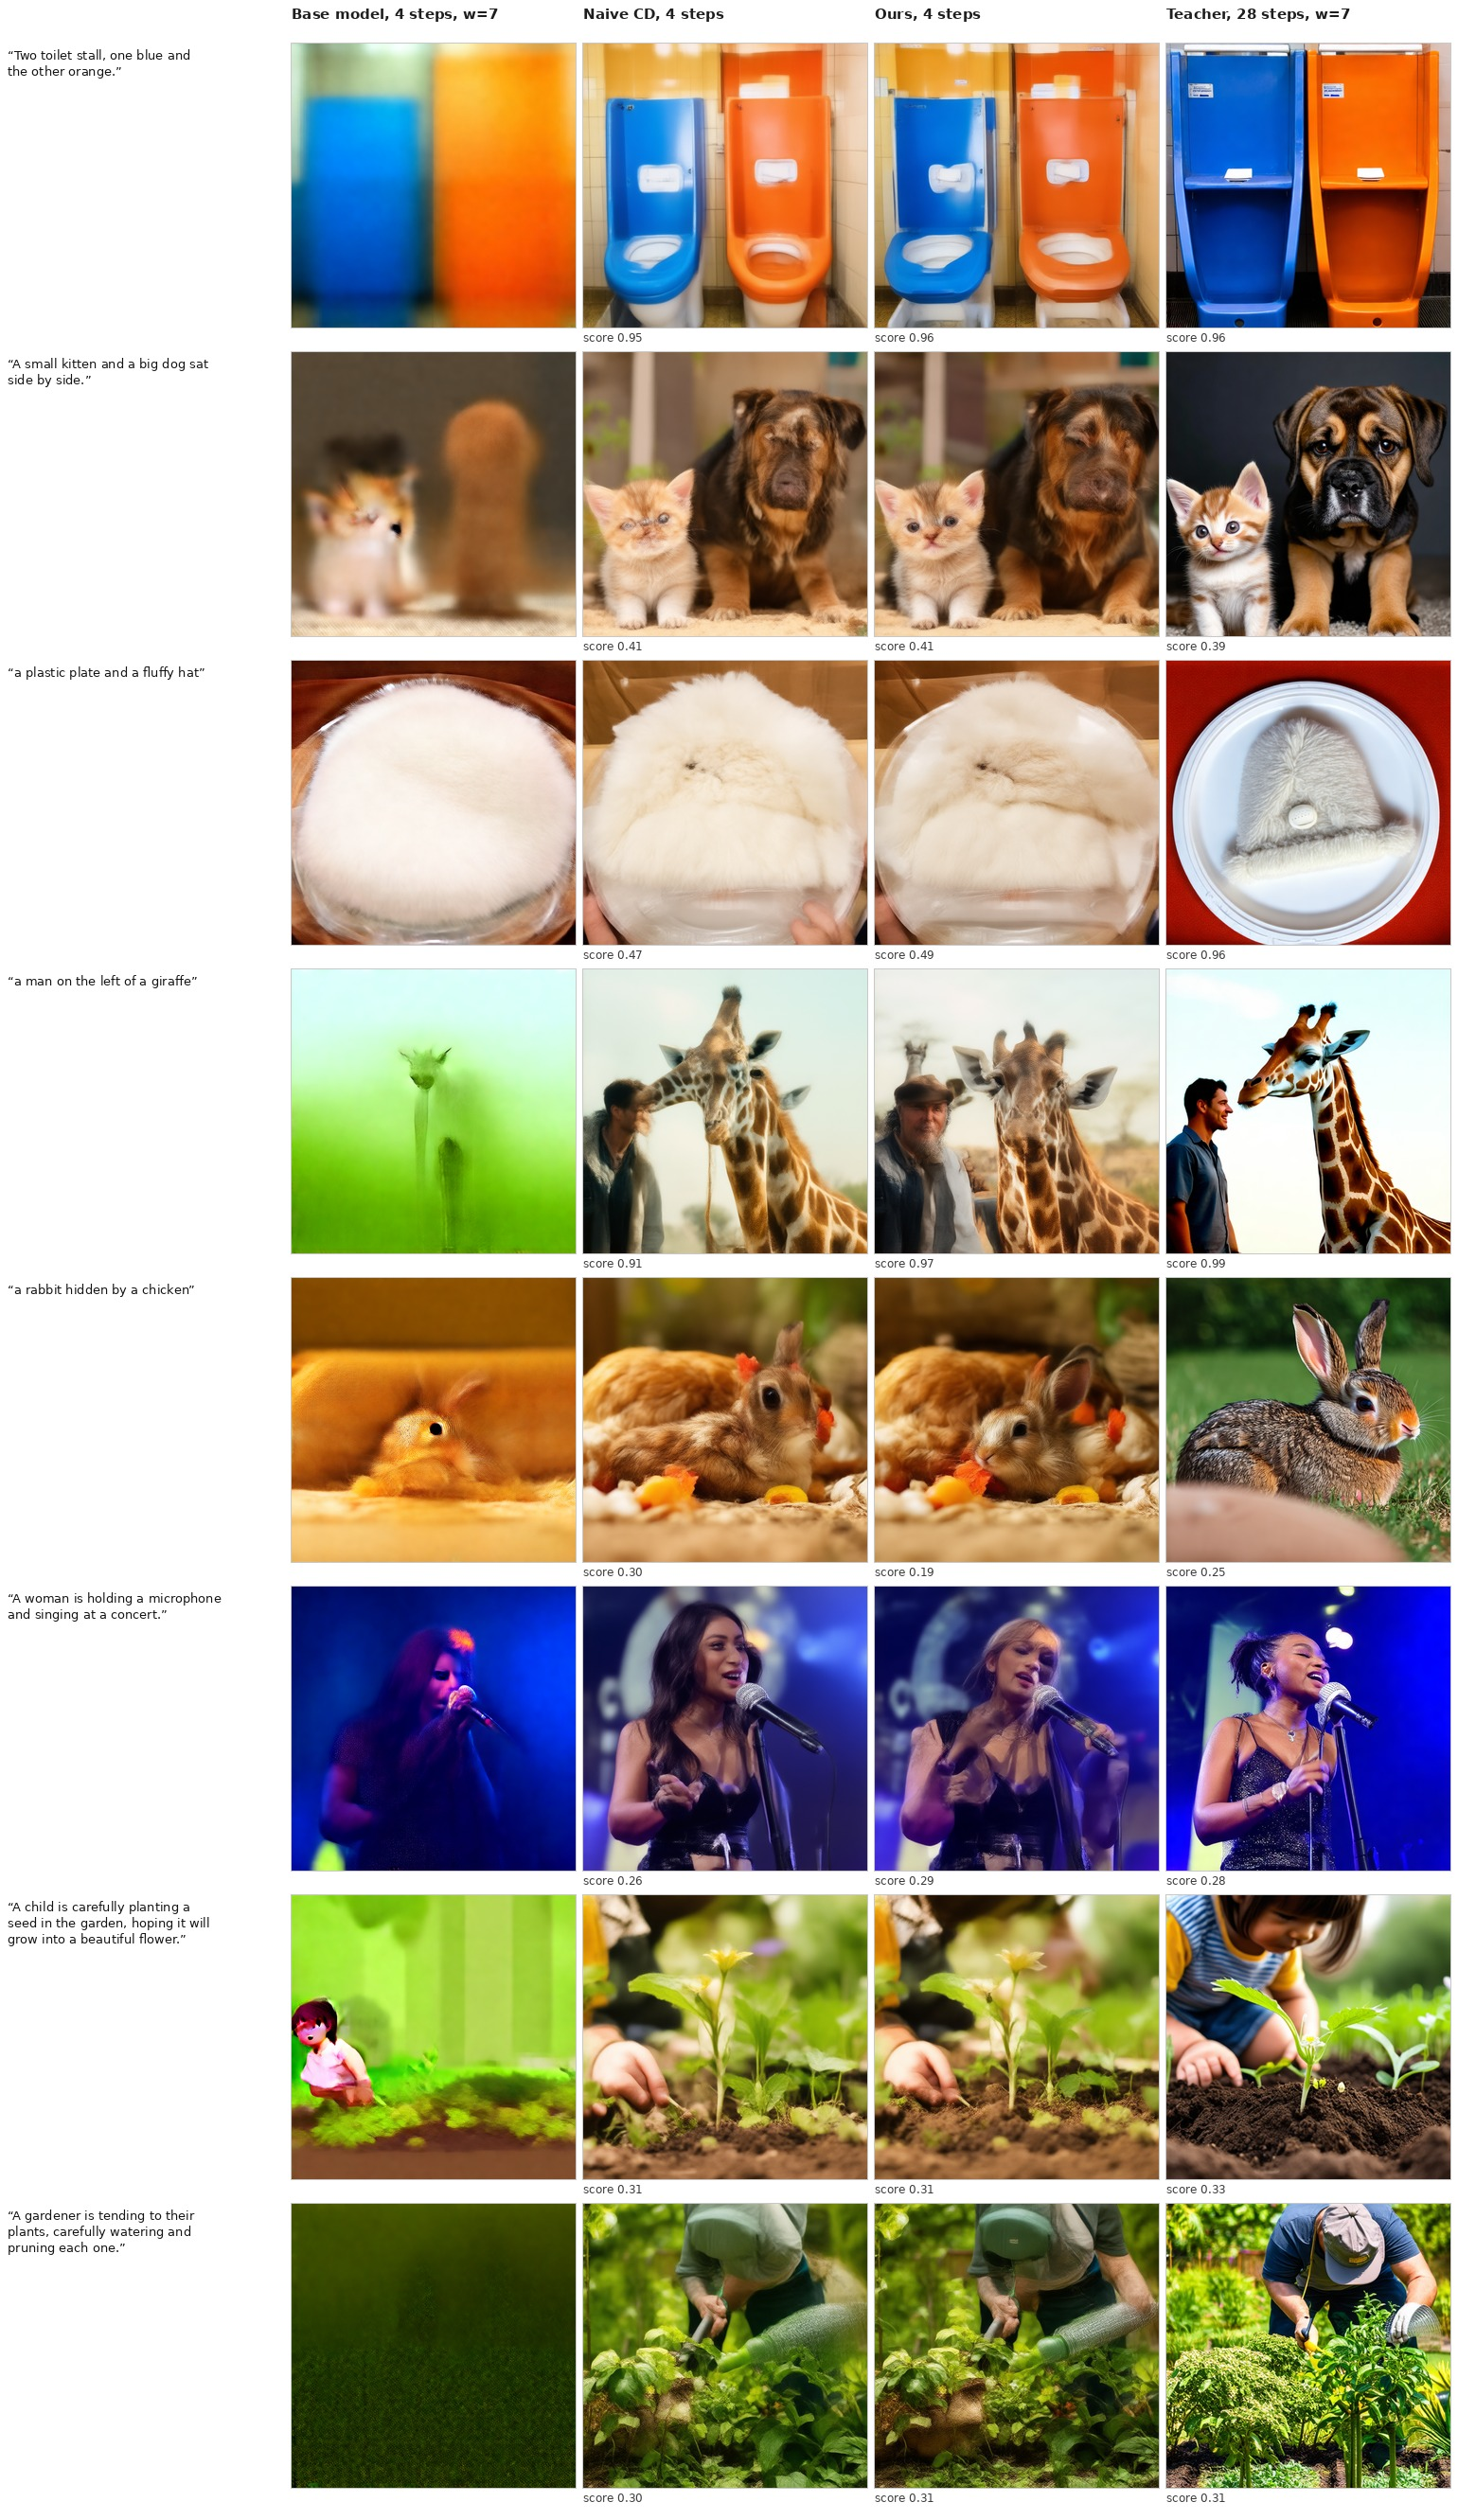
\includegraphics[width=\textwidth,height=0.68\textheight,keepaspectratio]{qual_uncurated_compbench.jpg}
\caption{Uncurated T2I-CompBench prompts (eight prompts drawn at random with a fixed seed). Columns share
the initial noise; scores are the official per-category evaluator's.}
\label{fig:unc-cb}
\end{figure}

\begin{figure}[p]
\centering
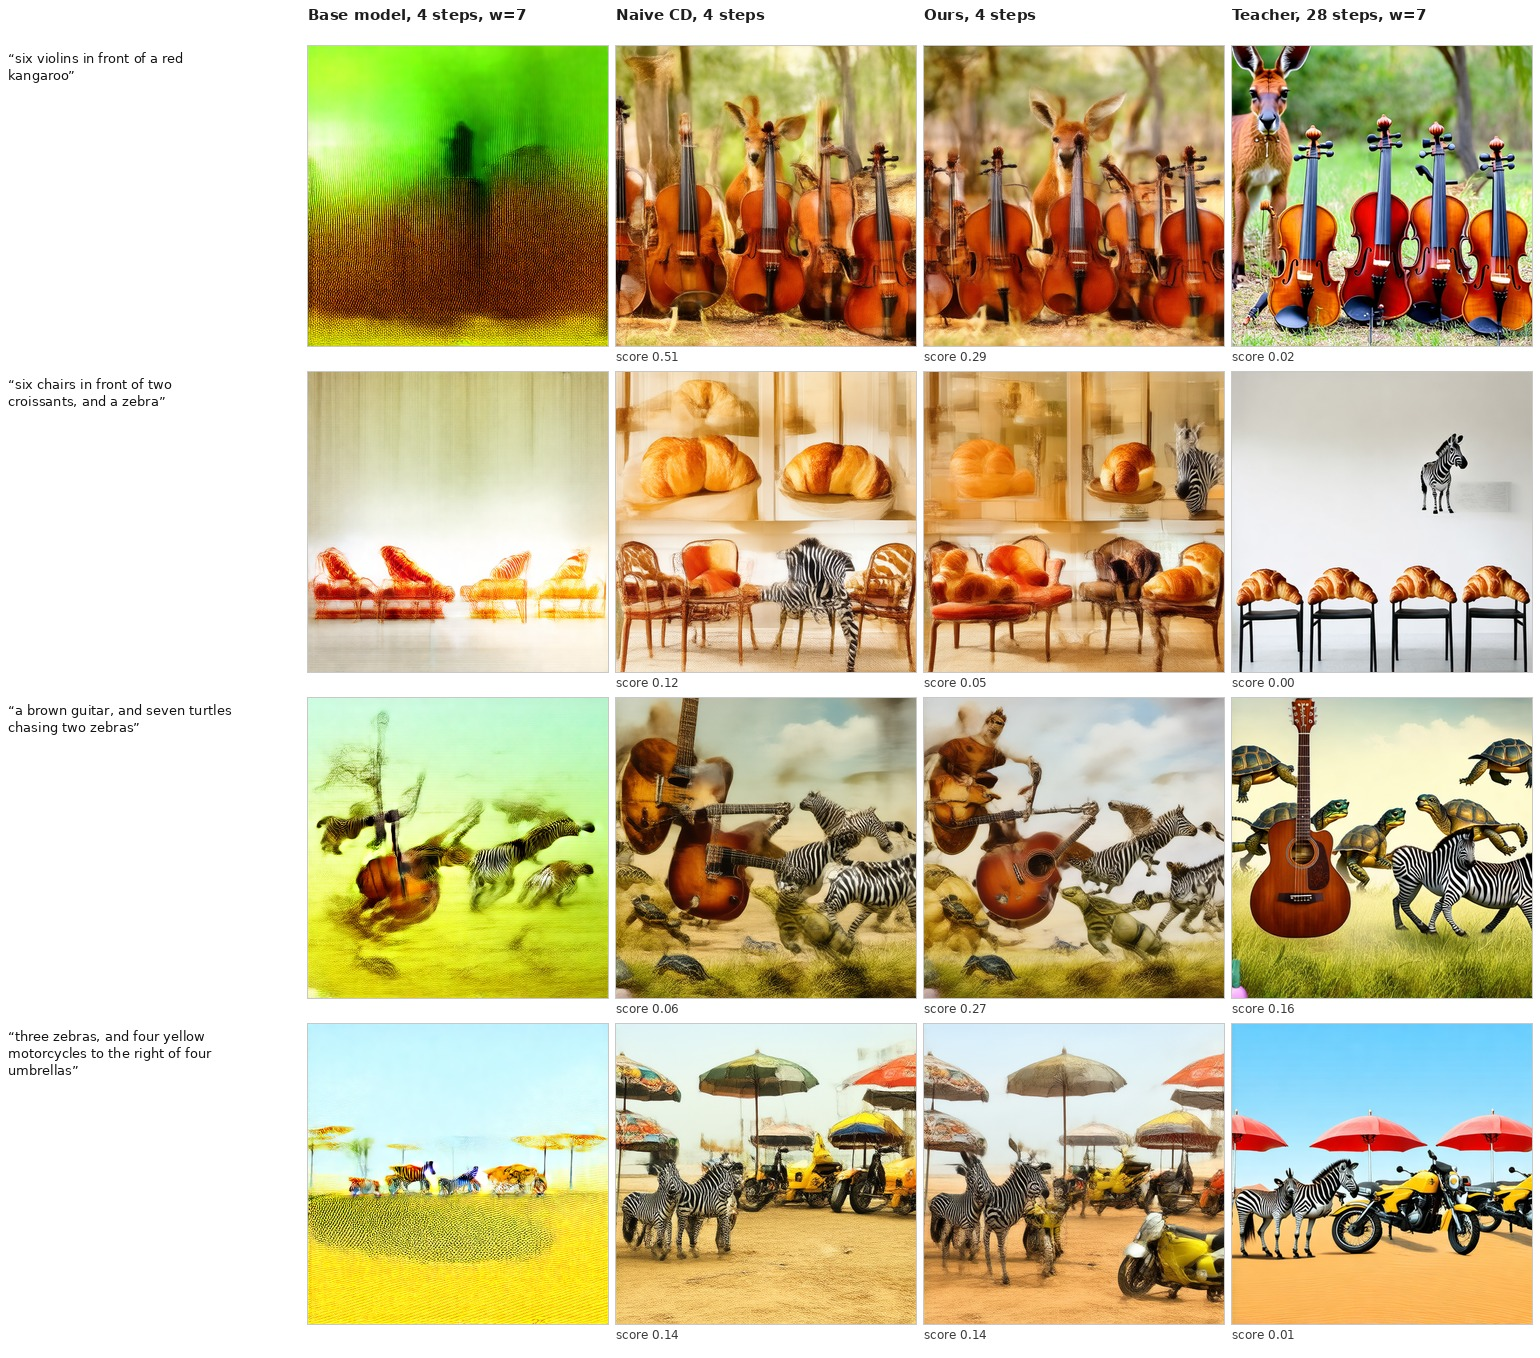
\includegraphics[width=\textwidth,height=0.42\textheight,keepaspectratio]{qual_uncurated_geneval2.jpg}
\caption{Uncurated GenEval2 prompts (four prompts drawn at random with a fixed seed).}
\label{fig:unc-ge}
\vspace{4mm}
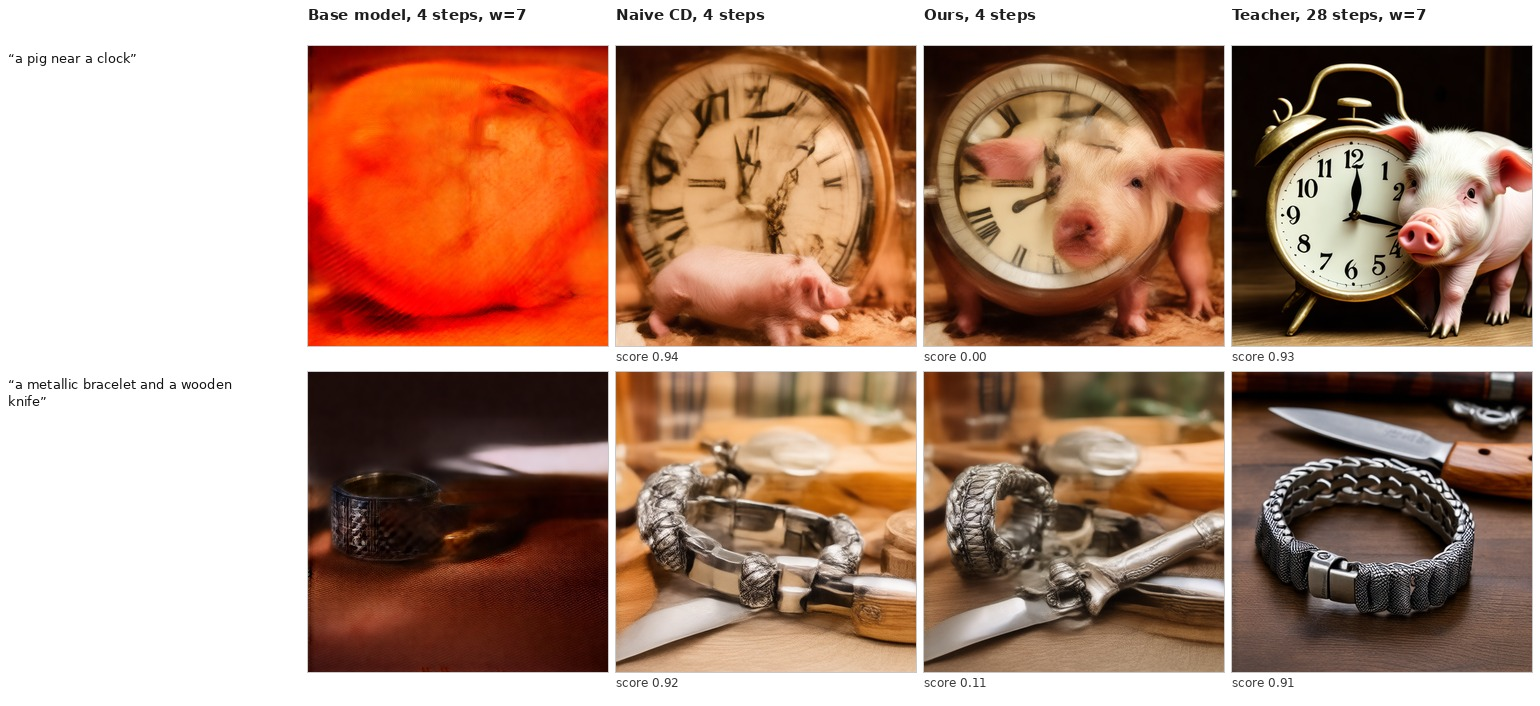
\includegraphics[width=\textwidth,height=0.2\textheight,keepaspectratio]{qual_regress_compbench.jpg}
\caption{The two T2I-CompBench prompts with the largest \naive{}-over-ours score margin.}
\label{fig:reg-cb}
\vspace{4mm}
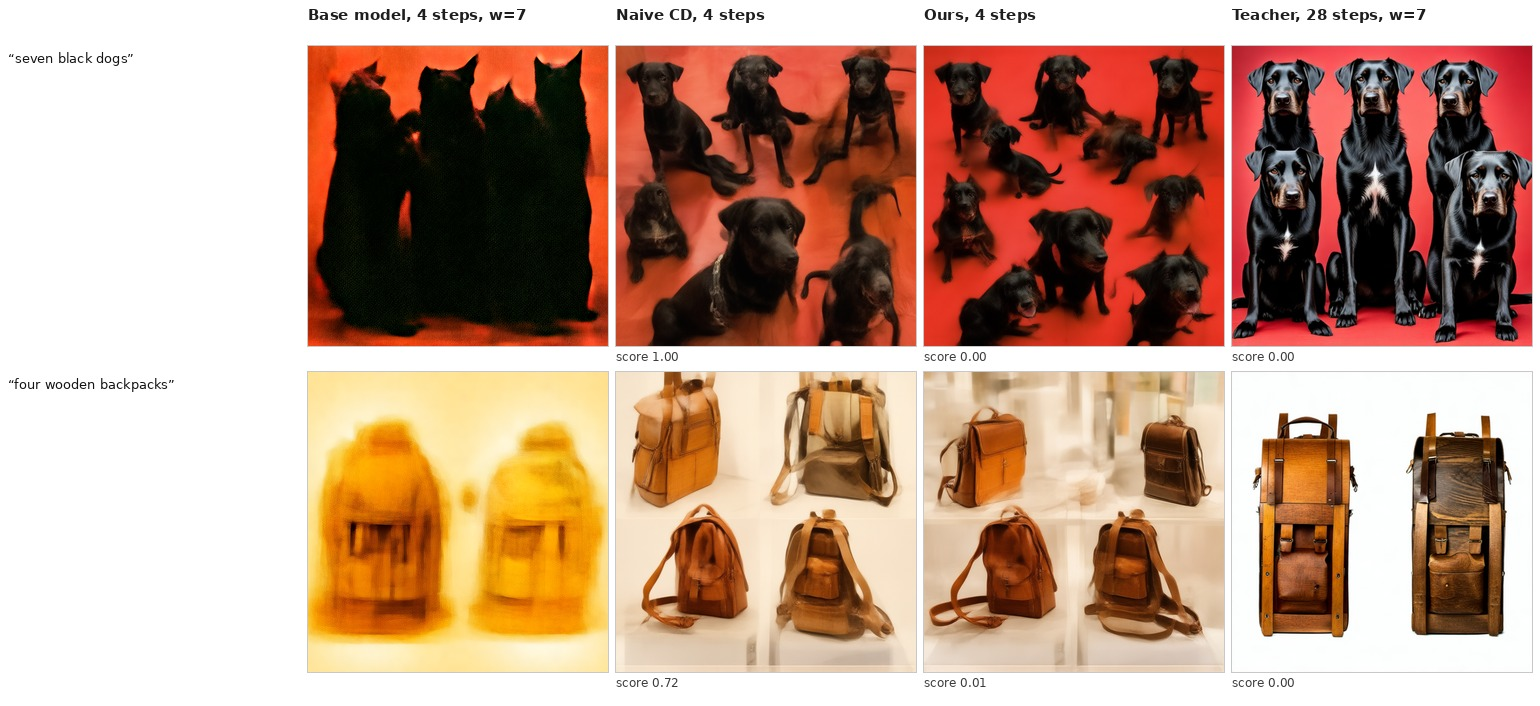
\includegraphics[width=\textwidth,height=0.2\textheight,keepaspectratio]{qual_regress_geneval2.jpg}
\caption{The two GenEval2 prompts with the largest \naive{}-over-ours score margin.}
\label{fig:reg-ge}
\end{figure}

\end{document}
